%!TEX root = ../iceDetection.tex

\documentclass[a4paper,14pt]{extarticle}

\usepackage{cmap}
\usepackage[T2A]{fontenc}
\usepackage[utf8x]{inputenc}
% \usepackage{mathptmx}
\usepackage[english, russian]{babel}

\usepackage{misccorr}
\usepackage{amssymb,amsfonts,amsmath,amsthm}  
\usepackage{indentfirst}
\usepackage[usenames,dvipsnames]{color} 
\usepackage[unicode,hidelinks]{hyperref}
\usepackage{makecell,multirow} 
\usepackage{ulem}
\usepackage{graphicx,wrapfig}
\graphicspath{{img/}}

\renewcommand{\labelenumii}{\theenumii)} 
\newcommand{\mean}[1]{\langle#1\rangle}

\DeclareMathOperator{\Div}{div}
\DeclareMathOperator{\const}{const}
%%%%%%%%%%%%%%%%%%%%%%%%%%%%%%%%%%%%%%%%%%%%%%%%%%%%%%%%%%%%%%%%%%%%%%%%%%%%%%%
%%%%%%%%%%%%%%%%%%%%%%%%%%%%%%%%%%%%%%%%%%%%%%%%%%%%%%%%%%%%%%%%%%%%%%%%%%%%%%%
\usepackage{float}
\usepackage[mode=buildnew]{standalone}
\usepackage[outline]{contour}
\usepackage{tocloft}
\renewcommand{\cftsecleader}{\cftdotfill{\cftdotsep}} % for parts
% \renewcommand{\cftchapleader}{\cftdotfill{\cftdotsep}} % for chapters
\usepackage{pgfplots,pgfplotstable,booktabs,colortbl}
\usepackage{physics}
\usepackage{mathtools}
% \mathtoolsset{showonlyrefs=true}

% \newcommand*\dotvec[1][1,1]{\crossproducttemp#1\relax}
% \def\crossproducttemp#1,#2\relax{{\qty[\vec{#1}\times\vec{#2}\,]}}

% \newcommand*\prodvec[1][1,1]{\crossproducttempa#1\relax}
% \def\crossproducttempa#1,#2\relax{{\qty[{#1}\times{#2}\,]}}
% \usepackage{showframe}
\usepackage[]{geometry}
\geometry{
  left=2.5cm,
  right=1.5cm,
  top=2cm,
  bottom=2cm,
  bindingoffset=0cm,
  headheight=17pt
}
\linespread{1.5} 
\setlength{\parindent}{1.25cm}
\frenchspacing 
\usepackage{setspace}
\setlength{\tabcolsep}{20pt}
\renewcommand{\arraystretch}{1.5}
\usepackage{xcolor}



\begin{document}

%!TEX root = ../iceDetection.tex
\begin{titlepage}
	\begin{center}
	  {\fontsize{ 12pt }{ 12pt } \selectfont \bf 
	  МИНИСТЕРСТВО НАУКИ И ВЫСШЕГО ОБРАЗОВАНИЯ \\[-10pt] 
	  РОССИЙСКОЙ ФЕДЕРАЦИИ}\\
	  \vspace{12pt}
	  \begin{spacing}{1}
		{\bf  Федеральное государственное автономное \\
		образовательное учреждение высшего образования \\
		<<Национальный исследовательский \\ 
		Нижегородский государственный университет им. Н.И. Лобачевского>>
		}
	  \end{spacing}
	  \vspace{24pt}
	  \begin{spacing}{1}
		Радиофизический факультет\\
		Кафедра общей физики\\
		\vspace{20pt}
		Направление <<Радиофизика>>\\
		\vspace{20pt}
		{ \fontsize{18pt}{18pt}ОТЧЕТ ПО УЧЕБНОЙ ПРАКТИКЕ}\\
		(Практика по получению первичных профессиональных умений и навыков, в том числе первичных умений и навыков научно-исследовательской деятельности\\
		% \vspace{20pt}
		% { \fontsize{18pt}{18pt} \bf Детектирование ледяного покрова по данным двухчастотного радиолокатора}
	  \end{spacing}
	  \vspace{100pt}
	  
		\begin{align*}
		  &\text{Руководитель практики:}\quad &\text{Панфилова М.\,А.}\\
		  &\text{Студент 3-го курса бакалавриата:}\quad &\text{Шиков А.\,П.}
		\end{align*}
	 
	\end{center}
	\vfill
	\begin{center}
	  {Нижний Новгород, 2019}
	\end{center}
  \end{titlepage}



\tableofcontents
\newpage
\section*{Введение}
\addcontentsline{toc}{section}{Введение}

Мониторинг ледяного покрова является важной задачей для решения как научных так и практических проблем. Он широко
применяется в мореходстве, предсказании изменений климата и погоды, а также для решения различных фундаментальных задач.
Спутниковое наблюдение обладает огромными возможностями в реализации мониторинга интересующих областей.
Это может быть оптическое наблюдение, например в ясную погоду лед хорошо виден с оптических снимков, однако во время
облачности этот способ по понятным причинам не подходит. Помимо оптики, используются пассивные методы радиометрии –
радиометры, и активные методы, такие как РСА и альтиметры. Однако исследованиями практически не охвачены, за исключением
альтиметра, диапазоны малых и средних углов падения от 0 $^{\circ}$ до 18$^{\circ}$.

В данной работе производится исследование методов детектирования льда на поверхности моря по данным для малых и средних углов падения,
используя данные двухчастотного радиолокатора, установленного на спутнике GPM (Global Precipitation Measurment).


\section{Миссия GPM}
Спутник миссии Global Precipitation Measurment был запущен в феврале 2014 для обнаружения  атмосферных осадков.
Он оборудован микроволновым формирователем изображений (GMI, радиометр), а также двухчастотным радаром (DPR). 

Радар работает в Ku(13.6 ГГц) и Ka(35.5 ГГц) диапазоне частот. Сканирование производится перпендикулярно направлению
полета, с максимальным отклонением до 18° у Ku диапазона, и до ??° у Ka диапазона. В таблице ?? приведена некоторая
техническая информация о радаре.
Ширина полосы обзора составляет 245 км, со средним разрешением 5 км.

Ku и Ka диапазоны радара выравнены, и при измерении области совпадают для двух частот. 

DPR и GMI - основные инструменты на спутнике GPM. С их помощью производится 3-х мерное наблюдение дождей в атмосфере Земли.   

В ходе нескольких исследований [??вставить ссылка на работы В.Ю., Маши ], было показано, что двухчастотный радар
чувствителен не только к осадкам, но и к типу отражающей поверхности.


\section{Теория}

\subsection{Измерения радара}
\begin{figure}[h!]
  \centering
  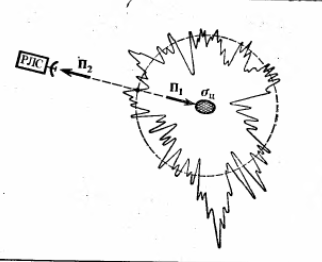
\includegraphics[width = .6\linewidth]{img/sigma0melnik.png}
  \caption{К формуле \eqref{eq:1.1}}
  \label{fig:1}
\end{figure}
Радар собирает информацию о величине сечения обратного рассеяния. 
Объект радиолокационного наблюдения можно охарактеризовать отношением напряженностей поля или плотностей потока мощности
отраженной волны и зондирующего колебания. В радиолокации характеристикой отражения сосредоточенной цели
является \textit{эффективная площадь}, или эффективная площадь рассеяния (ЭПР)\cite{meln}:
\begin{equation}
  \sigma = 4 \pi R^2 \frac{\Pi_2}{\Pi_1}
  \label{eq:1}
\end{equation}
Где $\Pi_1$ – плотность потока мощности падающей волны вблизи цели, а $\Pi_2$ – плотность потока мощности отраженной
волны, принятой РЛС, R - расстояние от РЛС до цели. (Множитель $4 \pi R^2$  исключает зависимость отношения плотностей потока от
расстояния.) ЭПР сильно зависит от формы, ориентации и материала облучаемого объекта. В нашем случае, когда тело имеет
большие размеры, имеет смысл ввода элементарной площадки S, и говорить не об эффективной площади, а об удельной
эффективной площади рассеяния, обозначаемой $\sigma^0$ (УЭПР) :
\begin{equation}
  \sigma^0 = 4 \pi R^2 \frac{\Pi_2}{S\Pi_1} = \gamma \cos \theta
  \label{eq:2}
\end{equation}
(Где угол $\theta$ – угол между направлением распространения и нормалью к площадке S.)

\subsection{Квазизеркальное приближение}
Если рассматривать с точки зрения теории, какую УЭПР должна иметь поверхность, например, воды, то наблюдаемое на
практике распределение достаточно хорошо описывается квазизеркальным приближением, в котором поверхность разбивается на
фасеты, и при отражении, вклад вносят только площадки, расположенные перпендикулярно к вектору падающей волны.


\begin{figure}[h!]
  \centering
  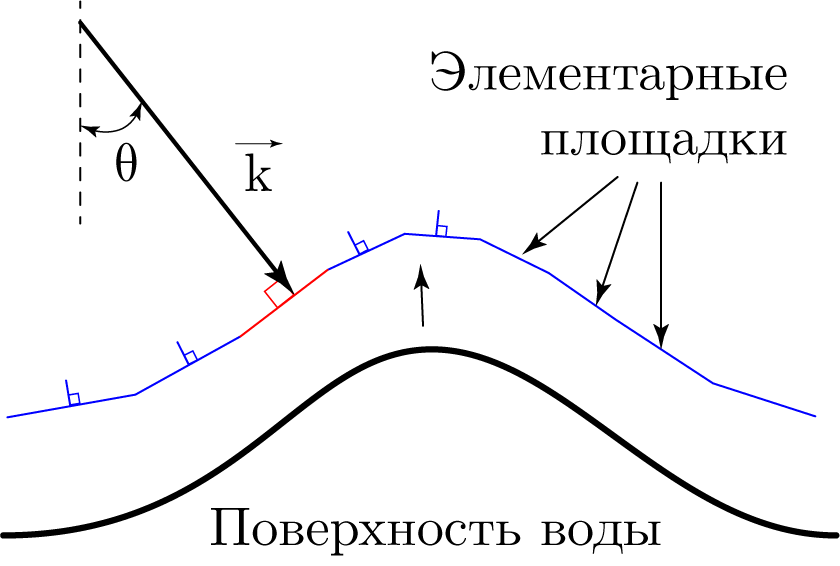
\includegraphics[width = .45\linewidth]{img/kvaz.png}
  \caption{}
  \label{fig:2}
\end{figure}
Для воды было проведено много теоретических исследований и экспериментов[??ссылку], в которых получено, что зависимость сечения рассеяния
от угла падения пропорциональна плотности распределения зеркальных площадок $P(\tan \theta)$:
\begin{equation}
  \sigma^0 = A (\cos \theta)^{-4} \cdot P(\tan \theta)
  \label{eq:3}
\end{equation}
, где $\theta$ - угол отклонения от нормали(А – эффективный коэффициент отражения, на величину которого влияет наличие
мелкой ряби). Для воды такая плотность имеет вид нормального распределения[??ссылку]:
\begin{equation}
  P_w(\tan \theta) = \frac{1}{\sigma_x \sqrt{2 \pi}} \cdot \exp (- \frac{\tan^2\theta}{2 \sigma^2_x})
  \label{eq:4}
\end{equation}
где $\sigma_x$ - что-то??

\subsection{Спутниковые данные}
Здесь приведен пример визуализации данных, полученных со спутника. Данные наложены на карту, а также приведен оптический
снимок за ту же дату. Цветом характеризуется величина сигнала – УЭПР в децибелах. (слайд) На снимке видно, что есть
прибрежная область, покрытая льдом, и через которую проходит трек спутниковых данных.
Мы можем взять эту область, и посмотреть какую угловую зависимость имеют срезы для разных типов поверхности. Здесь эти
срезы приведены на графике справа, и можно заметить, что наблюдается существенная разница между зависимостями для льда и
воды. Лед имеет большие значения при малых углах падения и малые значения при больших, в то время как вода имеет
достаточно плавное распределение. 
Зная, что поперечный срез льда имеет характерные отличия от воды, была сформулирована следующая задача: имея значение
УЭПР для поперечного среза, нужно определить, является ли облучаемый участок поверхности льдом, или нет.

Рассмотрим подробнее угловую зависимость для льда.  
Здесь приведены зависимости УЭПР в дэцибеллах от угла, собранные для некоторых сканов за период с января по март для 2017 года.
Как уже отмечалось, у льда зависимость имеет выделенный пик. Связано это с тем, что при околонулевом падении сигнала
отражение происходит преимущественно квазизеркально, и при увеличении угла характер меняется на диффузный. При нулевом
угле лед отражает большую энергию по сравнению с водой, так как на воде присутствует волнение и перпендикулярных к
падению сигнала площадок меньше, чем у льда. С ростом угла количество перпендикулярных площадок во льду резко падает, и
он приобретает характер диффузного рассеяния. Таким образом, зависимость УЭПР для льда выглядит как резкий пик. Чтобы
формализовать явно выраженную пикообразность, и использовать это как численный классификатор, можно использовать
коэффициент эксцесса.


Коэффициент эксцесса гамма 2 считается через четвертый центральный момент и дисперсию, при этом для гауссового
распределении, характерном для воды, этот коэффициент равняется нулю, т.е. для сканов воды он должен быть, может не
ноль, но очень мал. Для льда же, с сильно выделенным пиком, коэффициент эксцесса может быть не только не нулевым, но и
достаточно большим, что позволяет отличить лед при поперечном сканировании. 

Нам нужен коэффициент эксцесса плотности распределения, при известных значениях $\sigma_0$ и угла. В результате некоторых
пересчетов, мы можем, используя известные данные, а также нормировку плотности вероятности, рассчитать центральный
момент, а значит, коэффициент эксцесса для каждого поперечного среза. 

Если мы теперь построим эксцесс для каждого среза трека, то подтверждаются оба наших предположения: коэффициент эксцесса
для воды практически равен нулю, а для льда он значительно больше.



\section{Обработка данных}
\subsection{Алгоритм обнаружения льда}

\subsection{Детектирование границ}
Один из способов уточнить наше грубое приближение, это найти границы ледяного покрова.
Для определения границ необходимо детектировать скачки сигнала. Здесь приведены зависимости УЭПР от продольной
координаты для разных углов. Для того, чтобы выявить местонахождение скачка использовался алгоритм Джона Кэнни \cite{canny} для
одномерного случая.

\begin{equation}
  S = \frac{\left|\int \limits_{-W}^{+W} G(-x) f(x) d x\right|}{n_{0} \sqrt{\int \limits_{-W}^{+W} f^{2}(x) d x}} \frac{\left|\int \limits_{-W}^{+W} G^{\prime}(-x) f^{\prime}(x) d x\right|}{\sqrt{\int \limits_{-W}^{+W} f^{\prime 2}(x) d x}}
  \label{eq:S}
\end{equation}

\begin{equation}
  f(x) = -x\cdot \exp(-\frac{x^2}{2\sigma^2_g})
  \label{eq:fx}
\end{equation}

Рассмотрим для примера нулевой угол падения. Метод заключается в произведении двух сверток сигнала и
функции-детектора $f(x)$, результат которых здесь обозначен как S. В качестве функции-детектора выступала вторая производная от
Гауссового распределения.  Локальные максимумы функции S, соответствуют скачкам сигнала, или в нашем случае, переходам
между различающимися по характеру рассеивания поверхностями. Например здесь, первый максимум отвечает за переход
земля-лед, а второй, слабее – за переход лед-вода. 

На чувствительность алгоритма влияет вид функции-детектора, или здесь, в частности, ширина гауссового распределения
сигма. Важно, чтобы функция-детектор полностью убиралась в окно свертки, и при этом была достаточно, но не слишком
чувствительна. Чем уже функция-детектор, тем на меньшие скачки она реагирует, из-за чего функция S может стать очень
шумной. В работе был выбран оптимальный вариант соотношения ширины окна свертки и ширины функции, для наилучшего
детектирования. 

Используя такой подход обнаружения границ, размечался каждый продольный скан исследуемого трека. 

Имея теперь карту границ и карту расположения льда, мы можем совместить их, для получения более точной картины.
Например, мы можем заполнить ограниченную область, в соответствии с ее содержанием. Т.е. если в ограниченной области
находится преимущественно лед, то мы можем, учитывая что никаких скачков и перепадов там не происходило, заполнить всю
область льдом, и получить более правдоподобную разметку.

\subsection{Валидация}
Для валидации и исследования в работе использовались размеченные карты НИЦ «Планета», содержащие полигоны областей, и
информацию о них. Зная координаты точки, ее значение УЭПР и угла падения, а также полигона, в который она попадает, мы
сможем разметить наши данные для валидации после работы алгоритма. Также для валидации использовались данные с
радиометра, расположенного на том же спутнике. Однако для того, чтобы делать валидацию, нужно сначала сделать алгоритм,
к чему мы и переходим.  

Имея размеченные треки, мы можем сравнить их с данными радиометра, расположенного на том же спутнике, (слайд)а также с
картами планеты.

\section{Заключение}
Как видно, есть совпадение в общих чертах, но не обошлось и без пробелов. В основном это пропуски могут происходить при
попадании на срез нескольких типов поверхности. Все вышеописанные методы в таком случае работают на несколько порядков
хуже, или не работают вовсе. Чтобы детектировать лед в таких ситуациях, можно попытаться использовать машинное обучение,
для классификации поверхности в зависимости от уэпр, угла падения, и, например даты.

Ну и подведем итоги

В результате нашей работы был разработан алгоритм, позволяющий детектировать расположение ледяного покрова, используя
данные двухчастотного локатора спутника GPM для определения типа поверхности и границ.
Из очевидных недостатков, это неточная работа алгоритма при попадании на срез нескольких типов отражающей поверхности,
потому что в таком случае считать коэффициент эксцесса и производить аппроксимацию не имеет смысла. 
В перспективе имеется план использования этих данных для попытки реализации машинного обучения, однако это отдельная
тема, со своими проблемами и задачами, которые еще предстоит решить. 


\newpage
\addcontentsline{toc}{section}{Список литературы}
\begin{thebibliography}{99}
\bibitem{land} Ландау Л.Д., Лифшиц Е.М. Теоретическая физика: т.5, Статистическая физика. - М.: Физматлит, 2005. - 616 с.
\bibitem{dpr} GPM:DPR https://pmm.nasa.gov/gpm/flight-project/dpr.
\bibitem{meln} Мельник Ю.А., С.Г. Зубкович. Радиолокационные методы исследования Земли. ?? Советское радио, 1980 - 7 с.
\bibitem{canny} John Canny, A computational approach to edge detection. 1986.
\end{thebibliography}

\end{document}